\documentclass{article}

% Eshtetic packages -----------------------
\usepackage{geometry}
 \geometry{
 a4paper,
 total={170mm,257mm},
 left=25mm,
 right=25mm,
 top=25mm,
 bottom=25mm,
 }

 % A little black magic
\usepackage{microtype}

% Other Packages --------------------------

\usepackage{stmaryrd}
\usepackage{biblatex}
\usepackage[T1]{fontenc}
\usepackage{enumitem}

\usepackage{graphicx}
\graphicspath{ {../images/} }

\usepackage{caption}
\usepackage{subcaption}
\usepackage{amsthm}
\usepackage{amsmath}
\usepackage{amssymb}
\usepackage[french]{babel}
% \usepackage[autolanguage]{numprint} % for the \nombre command
\usepackage{hyphenat}
% \usepackage{minted}
% \setminted[ocaml]{style=vs}

\usepackage{tikz}

% Operators -------------------------------

\let\loop\relax
\DeclareMathOperator{\loop}{loop}
\DeclareMathOperator{\inv}{inv}
\DeclareMathOperator{\isconnected}{is-connected}
\DeclareMathOperator{\isgroupoid}{is-groupoid}
\let\Pr\relax
\DeclareMathOperator{\Pr}{Pr}
\DeclareMathOperator{\shape}{shape}
\DeclareMathOperator{\gset}{G-Set}
\DeclareMathOperator{\Torsor}{Torsor}
\DeclareMathOperator{\Aut}{Aut}
\DeclareMathOperator{\code}{code}
\DeclareMathOperator{\decode}{decode}
\DeclareMathOperator{\transport}{transport}
\DeclareMathOperator{\refl}{refl}
\DeclareMathOperator{\BAut}{BAut}

% \addbibresource{bibliographie.bib}

% \captionsetup{labelformat=empty}

%\renewcommand{\labelitemi}{$\bullet$}

\newtheorem{definition}{Définition}[section]
\newtheorem{proposition}[definition]{Proposition}
% \newtheorem{conjecture}[definition]{Conjecture}
% \newtheorem{exemple}[definition]{Exemple}


\title{Construction des espaces de Eilenberg-MacLane en HoTT}

\author{Stage L3 de Camil Champin}
\author{Camil Champin\\[1ex]
\small Encadré par Emile Oleon et Samuel Mimram}  % use a smaller font size
\date{Juin-Juillet 2023}

\begin{document}

\maketitle

\section{Introduction du problème}

% Ceci devrait s'écrire tout seul
%


\subsection{Notion de Groupe en HoTT}

\paragraph{Note sur les types connexes :} Dans un type connecté, tout les types égalité sont non-vides. Pour autant il ne s'agit pas toujours de propositions :

\[\prod_{x,y : X} \|x = y\|_{-1} \not\simeq \prod_{x,y : X} (x = y)\]

En particulier, une proposition (droite) a des égalités triviales, ce qui n' est pas le cas pour tout type connexe : un exemple est $\mathbb{S}_{1}$.

\begin{definition}

On appelle \emph{groupe} un tuple :

\begin{itemize}
        \item $S : Set$
        \item $e : S$
        \item $\mu : \displaystyle\sum_{\star : S \to S \to S} \displaystyle\prod_{g_1,g_2, g_3 : S} (g_1 \star e = e \star g_1 = g_1 ) \times (g_1 \star (g_2 \star g_3) = (g_1 \star g_2) \star g_3) $
        \item $\iota : \displaystyle\sum_{\inv : S \to S} \displaystyle\prod_{g : S} (f(g) \star g = g \star f(g) = e)$
\end{itemize}

\end{definition}


\subsection{Type Classifiant}

Une operation fréquente en théorie des catégories est de faire correspondre à chaque monoïde une catégorie pointée à \emph{un} objet, c'est à dire un point avec des flèches qui bouclent sur lui.

\begin{figure}[h]
\centering
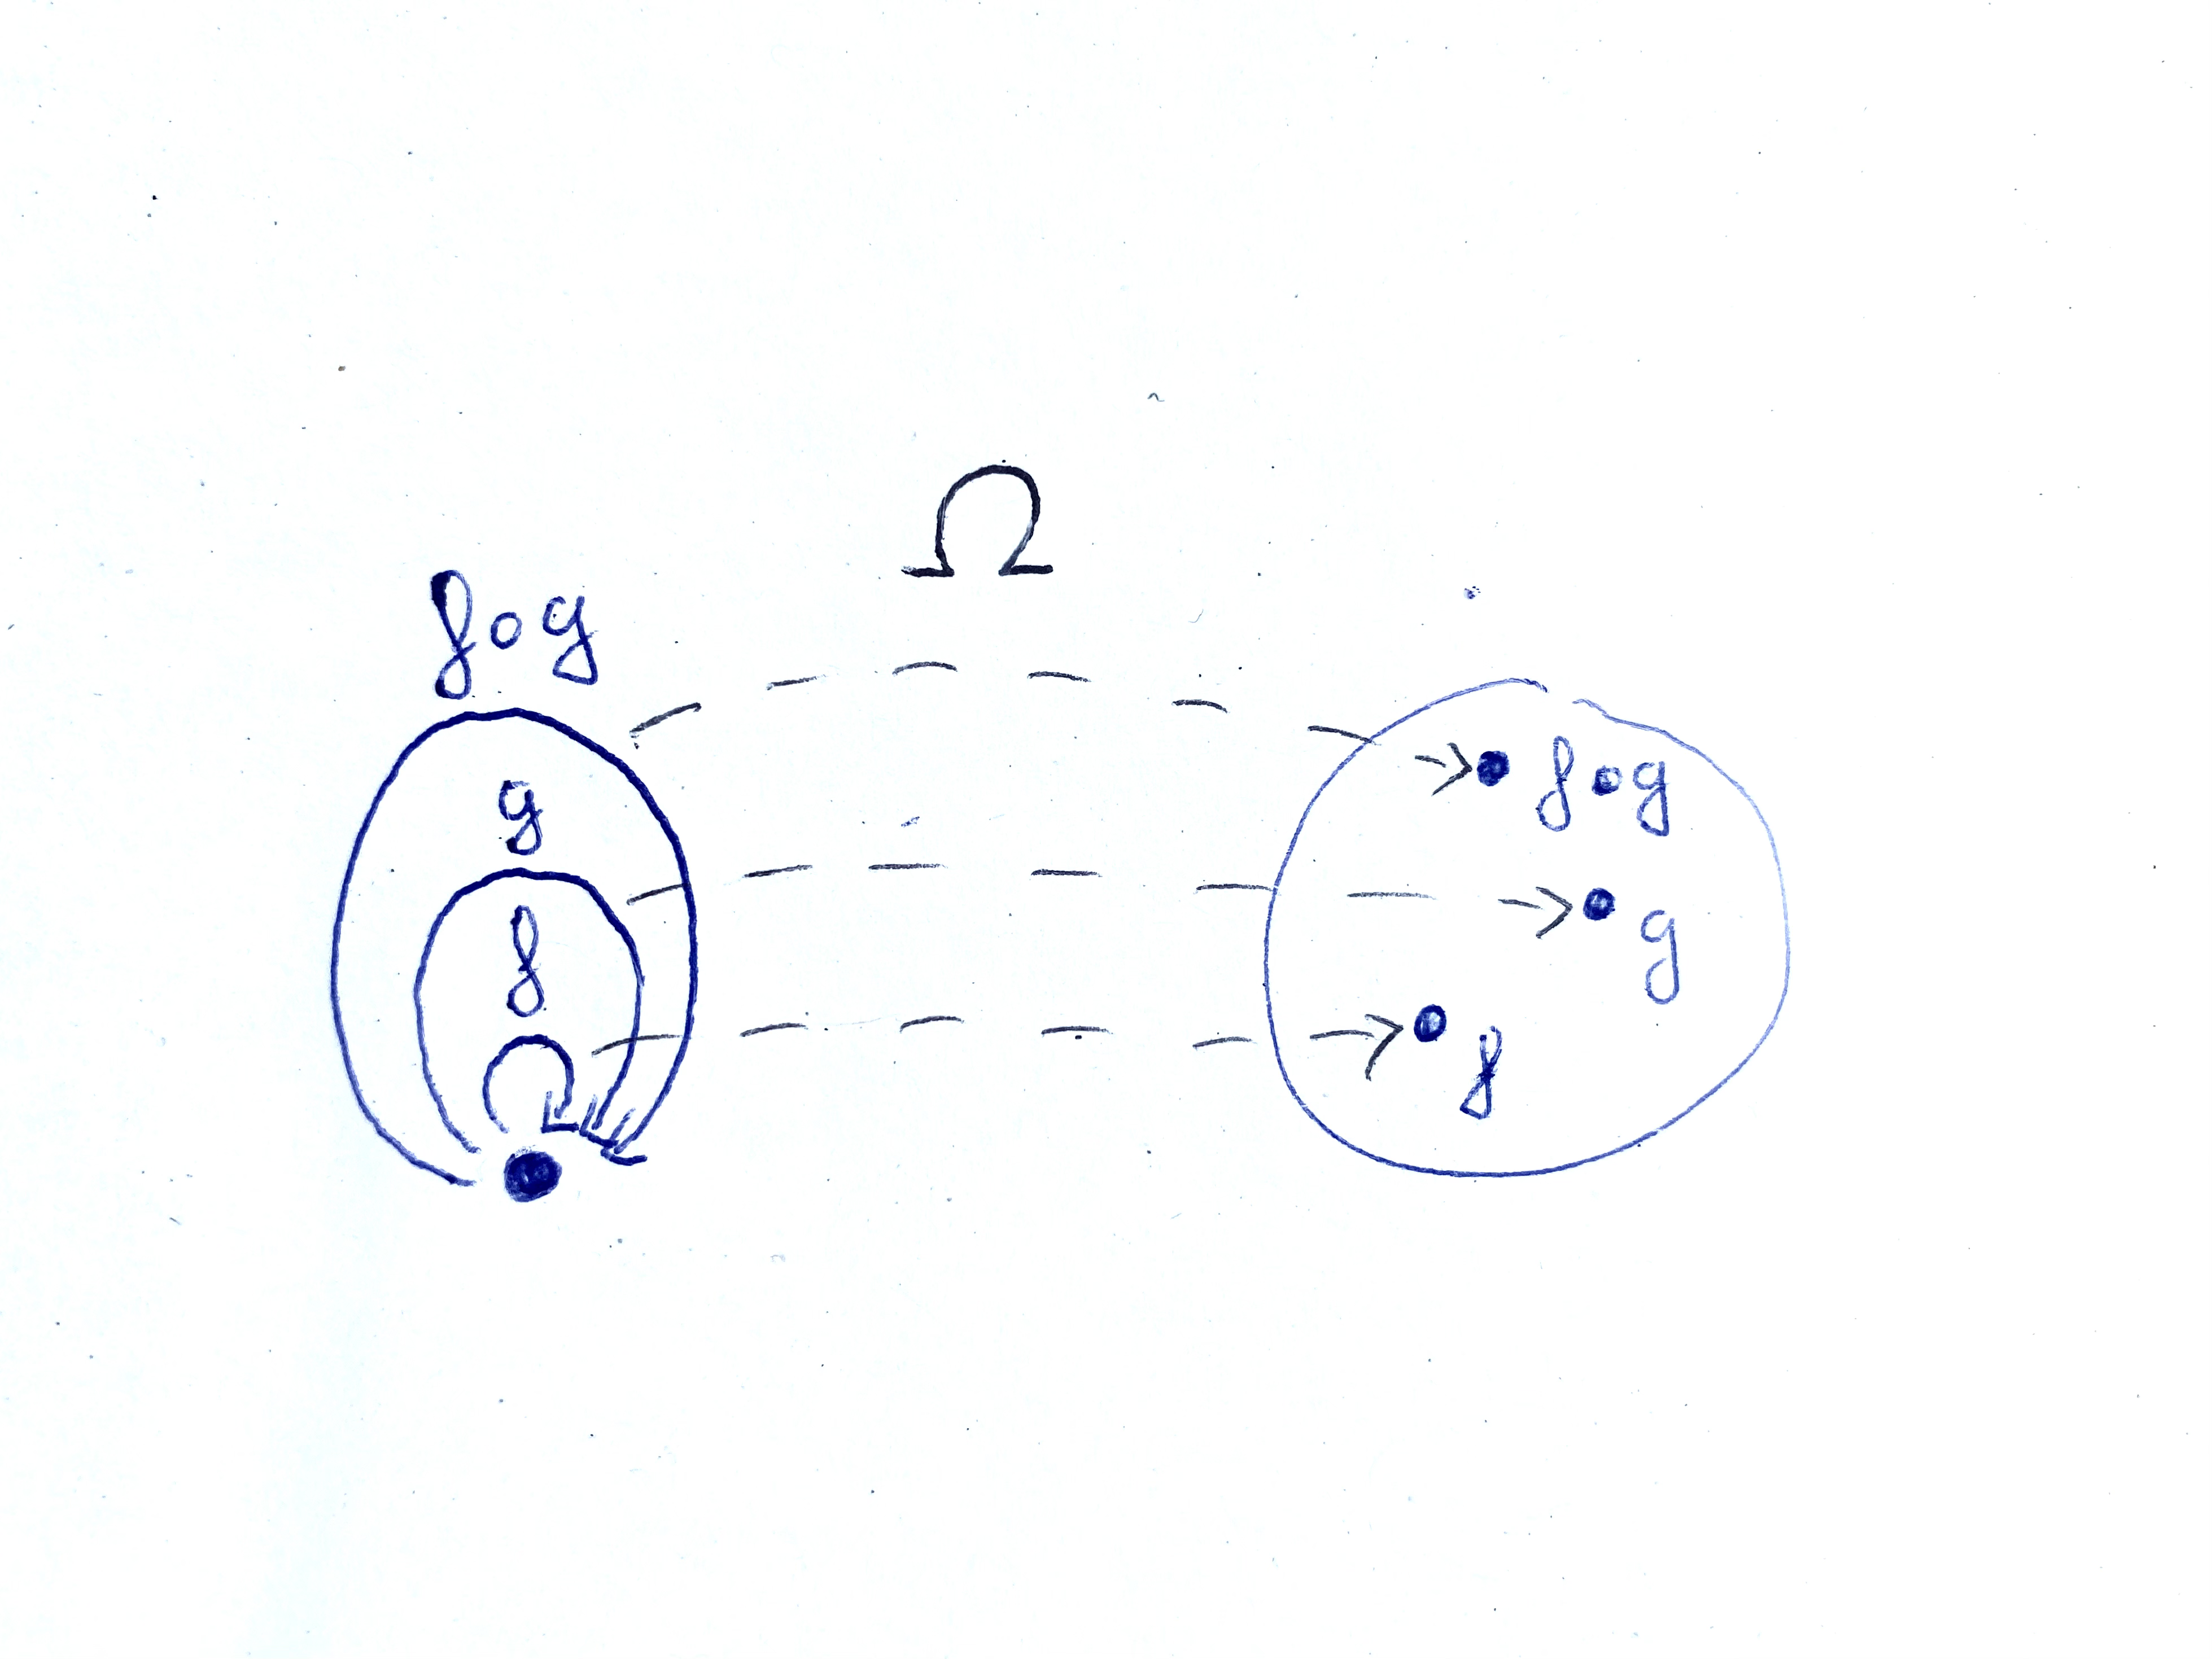
\includegraphics[scale=0.03]{omega}
\end{figure}

L'objet qui va jouer le rôle de la catégorie ici est un type \emph{non-vide}, \emph{connexe}, et on réclame également qu' il s'agisse d'un \emph{groupoïde} (les types égalité sont des ensembles). On pose l'univers de tels types :

\[\mathcal{U}_{*}^{=1} :\equiv \displaystyle\sum_{A : \mathcal{U}}A \times \isconnected(A) \times \isgroupoid(A)\]

Il s'agit d'un espace pointé $(A,a)$, son \emph{loop-space} $\Omega(A,a) :\equiv (a = a)$ est un ensemble, et c'est naturellement un groupe. On va enfaite montrer que cette transformation $\Omega$ est une équivalence, on appelle sa pseudo-inverse $B$. Ainsi pour chaque groupe $G$ on a un \emph{espace classifiant} de $G$, $BG$. On appelle $\shape_{G}$ l'élément distingué de $BG$.

\subsection{Actions de Groupes}

% On définit $BG$ comme le HIT suivant :

% \begin{itemize}
%         \item $* : BG$
%         \item $\loop : G \to *=*$
%         \item loop-composition $: \displaystyle\prod_{g,h : G} \loop(g \cdot h) = \loop(g) \cdot \loop(h)$
% \end{itemize}

Une action $\phi$ de $G \curvearrowright X$ est de la forme suivante :

\begin{gather*}
  \phi : BG \to Set \\
  * \mapsto X
\end{gather*}

De sorte à ce que par transport $\phi(g) : X = X$, à lire comme ``$\phi$ induit pour chaque élément de $G$ un automorphisme de X''. On note G-set : $(BG \to  Set)$ le type des ensembles sur lesquels $G$ agit.

\section{Construction de $K(G,1)$ par torseurs}

% \subsection{$BG$ est un $K(G,1)$}

% On remarque que $BG$ est un espace dont le groupe fondamental est $G$, et dont tout les autres groupes sont triviaux :

% \begin{itemize}
%   \item $\pi_{0}(BG) = 0$ par connexité.
%   \item $\pi_{1}(BG) = G$ car il s'agit de $\Omega BG$
%   \item $\pi_{n}(BG) = 0$ pour tout $n \geq 2$ car $\Omega BG$ est un ensemble.
% \end{itemize}

% Il s'agit à présent de construire BG. Pour cela, nous introduisons la notion de torseurs.

% \subsection{Notion de Torseur}

% On pose $BG$ tel que $\Omega BG :\equiv G$.

% \begin{definition}
%  on appelle \emph{torseur principal} de G :
%   \begin{gather*}
%     \Pr_{G} : BG \to Set \\
%     \Pr(x) :\equiv (\shape_{G} = x)
%   \end{gather*}
% \end{definition}

% Et on définit le type des torseurs :

% \[\Torsor_{G} :\equiv \sum_{X : \gset} \| X = \Pr_{G} \|_{-1}\]

\begin{definition}
  Si $(A,a_0)$ est un type pointé, on note $\BAut(A) :\equiv \sum_{x : A}\| x = a_{0} \|_{-1}$ la composante connexe de $a_0$ dans $A$.
\end{definition}

\begin{proposition}
  Le loop-space de la composante connexe de $a_0$ est le loop-space de $a_0$ :
  \[\Omega(\BAut(A)), a_0) = \Omega(A,a_0)\]
\end{proposition}

\begin{proof}
  $(\BAut(A), a_0)$ est un type pointé, et soit $\code$ la fibration :
  \begin{gather*}
    \code : \BAut(A)) \to \mathcal{U} \\
    (x,!) \mapsto (x =_{A} x)
  \end{gather*}
  On pose la fonction $\decode$ qui à $(x,!_{x})$ et $p : (x = a_0)$ associe un élément de $((x,!_{x}) = (a_0,!_{a_{0}})) \simeq \sum_{p : (x = a_0)}(p^{*}(!_{x}) = !_{a_0})$. Il suffit de donner un élément de ce second type. C'est un tuple, le premier élément est p, le second est une preuve de $(p^{*}(!_{x}) = !_{a_{0}})$ qu'on tire de la contractibilité de $\|a_0 = a_{0}\|_{-1}$. On vérifie les hypothèses du lemme encode-décode pour les loop-spaces :
  \begin{enumerate}
    \item $c_0 :\equiv \refl_{a_0} : \code(a_0)$
    \item $\decode : \prod_{x : \BAut(A)} \code(x) \to ((a_{0},!) = x)$
    \item Si $c : \code(a_0) \equiv (a_0 = a_0)$, alors $\decode_{a_0}(c) = ((a_{0},!) = (a_{0},!))$ et :\\
          $\transport^{\code}(\decode_{a_0}(c), c_0) = c_0 \equiv \refl_{a_0}$ par construction du transport.
    \item $\decode_{a_0}(c_0) = c_{0}$
  \end{enumerate}
\end{proof}


\section{Construction concise à partir de générateurs}

\subsection{Exemple des groupes cycliques}
\subsection{Généralisation}
\subsection{Exemple sur un autre groupe} % groupe dihédral ?
\subsection{Correction}

\end{document}
